
\section{Introduction}
%GPS units of a tractor working on an orchard could provide some information, including position, velocity, acceleration, etc, with which an orchardist is able to follow the trajectory and motion patterns of tractors. 

%The observed position data set $y_i$ always comes with some errors $\varepsilon_i$, which are assumed independent Gaussian distribution with variance $\sigma_n^2$. A popular method for finding $f(x)$ that fits these data is to augment/replace the vector of inputs $\mathbf{X}$ with additional variables, which are transformations of $\mathbf{X}$, and then use linear models in this new space of derived input features.\cite{esl2009}

In regression problem, linear regression, linear discriminant analysis, logistic regression and separating hyperplanes all rely on a linear model. With the good property of linear model, easy to be interpreted and first order Taylor approximation to $f(t)$, it is more convenient to represent $f(t)$ by linear model. However, the true function $f(t)$ is unlikely to be an actual linear function in space $\mathbb{R}$. Researchers found some methods for moving beyond linearity. One of them is replacing the vector of inputs $\mathbf{T}$ with its transformations as new variables, and then use linear models in this new space of derived input features.

Denote by $h_m(t):\mathbb{R} \mapsto \mathbb{R}$ the $m$th transformation of $t$, $m =1, \cdots ,M$. We then model
\begin{equation}\label{fbasis}
f(t) =\sum_{m=1}^{M}\beta_mh_m(t).
\end{equation}
a linear basis expansion of $\mathbf{t}$ in $\mathbb{R}$, where $h_m(t)$ are named basis functions, $\beta_m$ are coefficients. Once the basis functions $h_m$ have been determined, the models are linear in these new variables, and the fitting proceeds as before.

Suppose we are given observed data $t_1,t_2, \cdots, t_n$ on interval $[0,1]$, satisfying $0\leq t_1< t_2 < \cdots <t_n \leq 1$. A piecewise polynomial function $f(t)$ can be obtained by dividing the interval into contiguous
intervals $(t_1,t_2),\cdots,(t_{n-1},t_n)$, and representing $f$ by a separate polynomial in each interval. The points $t_i$ are called knots. For example,
\begin{equation}
f(t)=d_i(t-t_i)^3+c_i(t-t_i)^2+b_i(t-t_i)+a_i,
\end{equation}
for given coefficients $d_i, c_i, b_i$ and $a_i$, where $t_i\leq t\leq t_{i+1}$, $i=1,2,\cdots,n$. $f$ is a cubic spline on $[0,1]$ if (1) on each intervals $f$ is a polynomial; (2) the polynomial pieces fit together at knots $t_i$ in such a way that $f$ itself and its first and second derivatives are continuous at each $t_i$. If the second and third derivatives of $f$ are zero at 0 and 1, $f$ is said to be a natural cubic spline. These conditions are called natural boundary conditions.

Over all spline functions $f(t)$ with two continuous derivatives fitting these observed data, the curve estimate  $\hat{f}(t)$ will be defined to be the minimizer the following penalized residual sum of squares, \EDITED{edited expressions}
\begin{equation}\label{mse}
\text{MSE}(f,\lambda)=\frac{1}{n}\sum_{i=1}^n(f(t_i)-y_i)^2+\lambda \int_{0}^{1}(f''(t))^2dt
\end{equation}
where $\lambda$ is a fixed smoothing parameter, $(t_i,y_i)$, $i=1, \cdots, n$ are observed data and $0 \leq t_1< t_2 < \cdots <t_n \leq 1$. In equation (\ref{mse}),  the smoothing parameter $\lambda$ controls the trade-off between over-fitting and bias,
\begin{align}
\begin{cases}
\lambda = 0 : & \mbox{$f$ can be any function that interpolates the data,}\\
\lambda = \infty: & \mbox{the simple least squares line fit since no second derivative can be tolerated.}\\
\end{cases}
\end{align}

In our case, the velocity data set $v_i$ with some independent Gaussian distributed errors $\varepsilon_i \sim N(0, \frac{\sigma_n^2}{\gamma})$ are used to estimate $f(t)$ simultaneously. $f$ is a linear combination of basis functions, as shown in equation (\ref{fbasis}), in the meantime, $f'$ is a linear combination of the first derivative of these basis functions
\begin{equation}
f'(t) =\sum_{m=1}^{M}\alpha_mh'_m(t).
\end{equation}

The velocity information  is incorporated into MSE  equation (\ref{mse}) by the addition of velocity term $(f'(t_i)-v_i)^2$. Then it becomes 
\begin{equation}\label{mse2}
\text{MSE}(f,\lambda,\gamma)=\frac{1}{n}\sum_{i=1}^n(f(t_i)-y_i)^2+\frac{\gamma}{n} \sum_{i=1}^n(f'(t_i)-v_i)^2+\lambda \int_{0}^{1}(f''(t))^2dt,
\end{equation}
and $\hat{f}$ is the minimizer of the MSE equation (\ref{mse2}).

In the model $y=f(t)+\varepsilon$, it is reasonable to assume that the observed data $y_i$ is Gaussian distribution with mean $f(t_i)$ and variance $\sigma_n^2$. In a similar way, the velocity is estimated as  $v=f'(t)+\frac{\varepsilon}{\gamma}$, where $v_i$ is Gaussian distribution with mean $f'(t_i)$ and variance $\frac{\sigma_n^2}{\gamma}$. Then the joint distribution of $\mathbf{y},\mathbf{v},f(t)$ and $f'(t)$ is normal with zero mean and a covariance matrix, which can be estimated through Gaussian Process Regression.

\section{Gaussian Process Regression}

A Gaussian Process is a collection of random variables, any finite number of which have a joint Gaussian distribution, \cite{b_gpml}.

A GP is fully defined by its mean $m(t)$ and covariance $K(s,t)$ functions as
\begin{align}
m(t)&=\mathbb{E}[f(t)] \\
K(s,t)&=\mathbb{E}[(f(s)-m(s)) (f(t)-m(t))],
\end{align}
where $s$ and $t$ are two variables, and a function $f$ distributed as such is denoted in form of
\begin{equation}
f \sim GP(m(t),K(s,t)).
\end{equation}
Usually the mean function is assumed to be zero everywhere. 

Given a set of input variables $\mathbf{T}$ for function $f(t)$ and the output $\mathbf{y}=f(\mathbf{T})+\varepsilon$ with independent identically distributed Gaussian noise $\varepsilon$ with variance $\sigma_n^2$,  we can use the above definition to predict the value of the function $f_*=f(t_*)$ at a particular input $t_*$. As the noisy observations becoming
\begin{align}\label{covdef}
\text{cov}(y_p,y_q) = K(t_p,t_q)+\sigma_n^2 \delta_{pq}
\end{align}
where $\delta_{pq}$ is a Kronecker delta which is one iff $p=q$ and zero otherwise, the joint distribution of the observed outputs $\mathbf{y}$ and the estimated output $f_*$ according to prior is
\begin{equation}
\left[ \begin{matrix}
\mathbf{y}\\
f_*
\end{matrix} \right] \sim N \left(  
0,\left[   \begin{matrix}
K(\mathbf{T},\mathbf{T}) +\sigma_n^2I& K(\mathbf{T},t_*) \\
K(t_*,\mathbf{T}) & K(t_*,t_*)
\end{matrix}  \right] 
\right).
\end{equation}
The posterior distribution over the predicted value is obtained by conditioning on the observed data
\begin{equation}
f_* | \mathbf{y},\mathbf{T},t_* \sim N(\bar{f_*},\text{cov}(f_*))
\end{equation}
where 
\begin{align}
\bar{f_*}&=\mathbb{E}[f_* | \mathbf{y},\mathbf{T},t_* ]=K(t_*,\mathbf{T})[K(\mathbf{T},\mathbf{T})+\sigma_n^2I]^{-1}\mathbf{y},\\
\text{cov}(f_*)&=K(t_*,t_*)-K(t_*,\mathbf{T})[K(\mathbf{T},\mathbf{T})+\sigma_n^2I]^{-1}K(\mathbf{T},t_*).
\end{align}

We now add velocity information $\mathbf{v}=f'(\mathbf{T})+\varepsilon'$, where $\varepsilon'$ is independent distributed Gaussian noise with variance $\frac{\sigma_n^2}{\gamma}$.

It is expected that a position point $y_i$ and velocity point $v_i$ are all effected by other points $\mathbf{y}$ and $\mathbf{v}$. So the covariance matrix for $\mathbf{y}$ and $\mathbf{v}$ is
\begin{equation}\label{covYV}
\Sigma(\mathbf{y},\mathbf{v}) = 
\left[
\begin{matrix}
\text{cov}(\mathbf{y},\mathbf{y}) & \text{cov}(\mathbf{y},\mathbf{v}) \\
\text{cov}(\mathbf{v},\mathbf{y}) & \text{cov}(\mathbf{v},\mathbf{v}) 
\end{matrix}\right],
\end{equation}
where obviously $\text{cov}(\mathbf{y},\mathbf{v}) =\text{cov}(\mathbf{v},\mathbf{y})$. Then the joint distribution  is 
\begin{equation}
\left[
\begin{matrix}
\mathbf{y}\\
\mathbf{v}
\end{matrix}
\right] \sim N(\mu_{y,v},\Sigma_{y,v}).
\end{equation}
Define $f_*$ and $f'_*$ the estimated position and velocity values at point $t_*$. From equation (\ref{covYV}) and using similar idea, it is easily to get the covariance matrices 
\begin{equation}
\begin{split}
\Sigma(f_*,\mathbf{v}) &= 
\left[
\begin{matrix}
\text{cov}(f_*,f_*) & \text{cov}(f_*,\mathbf{v}) \\
\text{cov}(\mathbf{v},f_*) & \text{cov}(\mathbf{v},\mathbf{v}) 
\end{matrix}\right],\\
\Sigma(\mathbf{y},f'_*) &= 
\left[
\begin{matrix}
\text{cov}(\mathbf{y},\mathbf{y}) & \text{cov}(\mathbf{y},f'_*) \\
\text{cov}(f'_*,\mathbf{y}) & \text{cov}(f'_*,f'_*) 
\end{matrix}\right],\\
\Sigma(f_*,f'_*) &= 
\left[
\begin{matrix}
\text{cov}(f_*,f_*) & \text{cov}(f_*,f'_*) \\
\text{cov}(f'_*,f_*) & \text{cov}(f'_*,f'_*) 
\end{matrix}\right],
\end{split}
\end{equation}
\TODO{will need to give the form of these covariances at some point. in an appendix? i think you need discussion of how $f'$ is related to $f$ for a GP}

\section{A Reproducing Kernel in Space $\mathbb{H}$}\label{sectionRK}

$N_1(t), \cdots, N_n(t)$ denote $n$ basis function having first derivative in space $\mathbb{H}$. For any continuous function $f \in \mathbb{H}$, it is a combination of these basis functions
\begin{equation}
f(t)=\sum_{i=1}^{n} \alpha_iN_i(t),
\end{equation}
where $\alpha_i (i=1, \cdots, n)$ are coefficients. With an inner product
\begin{equation}\label{innerproduct}
\langle f,g\rangle= \langle\sum_{i=1}^{n} \alpha_iN_i(t), \sum_{i=1}^{n} \beta_iN_i(t)\rangle=\sum_{i=1}^{n} \alpha_i \beta_i, 
\end{equation}
it can be shown that the representer of evaluation $[s](\cdot)$ is
\begin{equation}\label{kernelfunction}
R_s(t) = \sum_{i=1}^{n} N_i(s)N_i(t),
\end{equation}
Then we can prove that the space $\mathbb{H}$ is a Reproducing Kernel Hilbert Space. In fact,
\begin{align}
\langle f(t), R(s,t)\rangle=\langle\sum_{i=1}^{n} \alpha_iN_i(t),  \sum_{i=1}^{n} N_i(s)N_i(t)\rangle=\sum_{i=1}^{n}\alpha_iN_i(s)=f(s).
\end{align}
The term $R(s,t)=R_s(t)$ is called the reproducing kernel function.


We now introduce a new notation $\dot{R}(s,t)$ in the following and use it to find the covariance matrix $\Sigma$ of the joint distribution of $\mathbf{y}, \mathbf{v}, f$ and $f'$.

Define $\dot{R}(s,t)$ and $R'(s,t)$ are the first partial derivative of $R(s,t)$ with respect to the first  and second argument respectively
\begin{align} \label{dotr}
\dot{R}(s,t)=\frac{\partial R(s,t)}{\partial s}=\sum_{i=1}^{n} \frac{dN_i(s)}{ds}N_i(t)=\sum_{i=1}^{n} N'_i(s)N_i(t),\\
\label{dotr2}
 R'(s,t)=\frac{\partial R(s,t)}{\partial t}=\sum_{i=1}^{n} N_i(s)\frac{dN_i(t)}{dt}=\sum_{i=1}^{n} N_i(s)N'_i(t),
\end{align}
Then $\dot{R}'(s,t)$ is the second partial derivative of $R(s,t)$ with respect to both arguments
\begin{equation}
\dot{R}'(s,t)=\frac{\partial^2 R(s,t)}{\partial s \partial t}=\sum_{i=1}^{n} \frac{dN_i(s)}{ds}\frac{dN_i(t)}{dt}=\sum_{i=1}^{n} N'_i(s)N'_i(t).
\end{equation}
It is easy to prove that $\dot{R}(s,t)=R'(t,s)$ and
\begin{equation}
\begin{split}
\langle f(t), R'(s,t)\rangle = \langle\sum_i \alpha_i N_i(t), \sum_i N_i(s)N'_i(t)\rangle =   \sum_i \alpha_i N_i(t) =f(t),\\
%\langle f'(t), \dot{R}(s,t)\rangle = \langle\sum_i \alpha_i N'_i(t), \sum_i N'_i(s)N_i(t)\rangle =   \sum_i \alpha_i N'_i(s) =f'(s),\\
%\langle f'(t), \dot{R}'(s,t)\rangle = \langle\sum_i \alpha_i N_i(t), \sum_i N'_i(s)N'_i(t)\rangle =   \sum_i \alpha_i N'_i(s) =f'(s),\\
\langle f(t),\dot{R}(s,t)\rangle = \langle \sum_i \alpha_i N_i(t), \sum_i N'_i(s)N_i(t)\rangle =   \sum_i \alpha_i N'_i(s) =f'(s),\\
%\langle R'(s,t),f'(t)\rangle = \langle\sum_i N_i(s)N_i'(t), \sum_i \alpha_i N'_i(t)\rangle =   \sum_i \alpha_i N_i(s) =f(s).
\end{split}
\end{equation}

Given the sample points $t_i, i=1, \cdots, n$ and noting that the space
\begin{equation}
\mathbb{A}=\{f: f=\sum_{i=1}^{n}\alpha_iR(t_i,\cdot) \} 
\end{equation}
is one linear subspace of $\mathbb{H}$. Then $f \in \mathbb{H}$ can be written as
\begin{equation}\label{etaeq}
f(t)=\sum_{i=1}^{n}c_iR(t_i,t)+\rho(t)
\end{equation}
where $c_i$ are coefficients, $\rho(t) \in \mathbb{H} \ominus \mathbb{A} $, and 
\begin{equation}\label{etaeq2}
f'(t)=\sum_{i=1}^{n}c_iR'(t_i,t)+\rho'(t).
\end{equation}

The equation (\ref{mse2}) can be written inform of
\begin{equation}
\begin{split}
\frac{1}{n}\sum_{i=1}^n (y_i -\sum_{j=1}^{n}c_jR(t_j,t_i) -\rho(t_i))^2+
\frac{\gamma}{n}\sum_{i=1}^n (v_i -\sum_{j=1}^{n}c_jR'(t_j,t_i) -\rho'(t_i))^2 \\
+\lambda \int_{0}^{1} (\sum_{j=1}^{n}c_jR''(t_j,t)+\rho''(t))^2dt
\end{split}
\end{equation}
As $\dot{R}(t_i,\cdot) = \sum_{j=1}^{n}N_j'(t_i)N_j(t) \in \mathbb{A}$, then by orthogonality and property of reproducing kernel functions, $\rho(t_i)=\langle R(t_i,\cdot),\rho\rangle=0$, %$\rho(t_i) =\langle\rho,R'(\cdot,t_i)\rangle=\langle\dot{R}(t_i,\cdot),\rho\rangle=0$, 
and $\rho'(t_i)=\langle \rho,\dot{R}(t_i,\cdot)\rangle=0$, where $i=1,\cdots,n$. 

Denoting by $Q$ the $n \times n$ matrix with the $(i,j)$th entry $R(t_i,t_j)$, by $P$ the $n \times n$ matrix with the $(i,j)$th entry $\dot{R}'(t_i,t_j)$ the equation (\ref{mse2}) can be written as
\begin{equation}\label{matrixeqc}
(\mathbf{y}-Q\mathbf{c})^\top(\mathbf{y}-Q\mathbf{c})+\gamma (\mathbf{v}-P\mathbf{c})^\top(\mathbf{v}- P\mathbf{c})+n\lambda \Omega+\lambda(\rho,\rho).
\end{equation}
Note that $\rho$ only appears in the third term in $(\ref{matrixeq})$, which is minimized at $\rho=0$. Hence, a polynomial smoothing spline resides in the space $\mathbb{A} $ of finite dimension. Then, following the method given from \cite{gubook}, the solution can be computed via minimization of term in $(\ref{matrixeqc})$ with respect to $\mathbf{c}$

\section{Covariance Matrix and Posterior Mean}\label{secmatrixandmean}

Consider $f$ and $f'$ in $\mathbb{H}$, having Gaussian priors with zero mean. By equation  (\ref{covdef}), their covariance functions are
\begin{equation}
\begin{split}
\text{cov}(f(s),f(t))&=\tau^2 R(s,t)+\sigma_n^2I\\
\text{cov}(f(s),f'(t))&=\tau^2 R'(s,t)+\frac{\sigma_n^2}{\sqrt{\gamma}}I\\
\text{cov}(f'(s),f(t))&=\tau^2 \dot{R}(s,t)+\frac{\sigma_n^2}{\sqrt{\gamma}}I\\
\text{cov}(f'(s),f'(t))&=\tau^2 \dot{R}'(s,t)+\frac{\sigma_n^2}{\gamma}I
\end{split}
\end{equation}
Observing $y_i \sim N(f(t_i),\sigma_n^2)$ and $v_i \sim N(f'(t_i),\frac{\sigma_n^2}{\gamma})$, the joint distribution of $\mathbf{y}, \mathbf{v}, f(t)$ and $f'(t)$ is normal with zero mean and covariance matrix
\begin{equation}\label{covyvff}
\begin{split}
\text{cov}(\mathbf{y},\mathbf{v},f,f') &= 
\left[ \begin{matrix}
\tau^2R(t_i,t_j)+\sigma_n^2I & \tau^2R'(t_i,t_j)+\frac{\sigma_n^2}{\sqrt{\gamma}}I & \tau^2R(t_i,t)& \tau^2R'(t_i,t) \\
\tau^2 \dot{R}(t_i,t_j)+\frac{\sigma_n^2}{\sqrt{\gamma}}I & \tau^2 \dot{R}'(t_i,t_j)+\frac{\sigma_n^2}{\gamma}I & \tau^2 \dot{R}(t_i,t)& \tau^2\dot{R}'(t_i,t)  \\
\tau^2R^\top(t_i,t) & \tau^2\dot{R}^\top(t_i,t) & \tau^2R(t,t)& \tau^2R'(t,t) \\
 \tau^2R'^\top(t_i,t)& \tau^2\dot{R}'^\top(t_i,t)& \tau^2\dot{R}(t,t)& \tau^2\dot{R}'(t,t)  \\
\end{matrix} \right] \\
&=
\left[ \begin{matrix}
\tau^2Q+\sigma_n^2I & \tau^2 O+\frac{\sigma_n^2}{\sqrt{\gamma}}I & \tau^2\xi & \tau^2\xi' \\
\tau^2 O+\frac{\sigma_n^2}{\sqrt{\gamma}}I & \tau^2 P+\frac{\sigma_n^2}{\gamma}I & \tau^2 \dot{\xi}& \tau^2\dot{\xi}' \\
\tau^2\xi^\top & \tau^2\dot{\xi}^\top & \tau^2R(t,t)& \tau^2R'(t,t) \\
 \tau^2\xi'^\top& \tau^2\dot{\xi}'^\top& \tau^2\dot{R}(t,t)& \tau^2\dot{R}'(t,t)  \\
\end{matrix} \right]
\end{split}
\end{equation}
where $\{Q\}_{ij}$ is the matrix with elements $R(t_i,t_j)$,  $\{O\}_{ij}$ is the matrix with elements $\dot{R}(t_i,t_j)=R'(t_j,t_i)$,  $\{P\}_{ij}$ is the matrix with elements $\dot{R}'(t_i,t_j)$, $\xi$ is a $n \times 1$ matrix with $i$th elements $R(x_i,x)$, and $\dot{\xi}$ is a $n \times 1$ matrix with $i$th elements $\dot{R}(x_i,x)$. Then
\begin{equation}
\begin{split}
E\left[ \begin{matrix}
f \\
f'
\end{matrix} | \begin{matrix}
\mathbf{y} \\
\mathbf{v}
\end{matrix}\right] &= 
\left[ \begin{matrix}
\xi^\top& \dot{\xi}^\top \\
\xi'^\top & \dot{\xi}'^\top 
\end{matrix} \right] 
\left[ \begin{matrix}
Q+n\lambda I & O+\frac{n\lambda}{\sqrt{\gamma}}I\\
 O+\frac{n\lambda}{\sqrt{\gamma}}I &  P+\frac{n\lambda}{\gamma}I
\end{matrix} \right]^{-1}
\left[ 
\begin{matrix}
\mathbf{y} \\
\gamma \mathbf{v}
\end{matrix} \right] \\
&\triangleq
\left[ \begin{matrix}
\xi^\top& \dot{\xi}^\top \\
\xi'^\top & \dot{\xi}'^\top 
\end{matrix} \right] 
\left[ \begin{matrix}
A & B\\
C & D
\end{matrix} \right]
\left[ 
\begin{matrix}
\mathbf{y} \\
\gamma \mathbf{v}
\end{matrix} \right] \\
&=
\left[ \begin{matrix}
\xi^\top(A\mathbf{y}+B\gamma \mathbf{v})+ \dot{\xi}^\top(C\mathbf{y}+D\gamma \mathbf{v}) \\
\xi'^\top(A\mathbf{y}+B\gamma \mathbf{v})+ \dot{\xi}'^\top(C\mathbf{y}+D\gamma \mathbf{v}) 
\end{matrix} \right] 
\end{split}
\end{equation}
where $n\lambda = \sigma_n^2 / \tau^2$. The posterior mean $E(f | \mathbf{y},\mathbf{v})$ is a linear combination of basis functions $N_i(t)$, and both $\xi$ and $\dot{\xi}$ contain $N_i(t)$, thus the posterior mean is of the form $\xi^\top \mathbf{c}+\dot{\xi}^\top\mathbf{d}$. Similarly, $E(f' | \mathbf{y},\mathbf{v})$ is of the form $\xi'^\top \mathbf{c}+\dot{\xi}'^\top\mathbf{d}$, with the same coefficients given by
\begin{align}
\mathbf{c}&=A\mathbf{y}+B\gamma \mathbf{v}\\
\mathbf{d}&=C\mathbf{y}+D\gamma \mathbf{v} 
\end{align}


\section{A 1-D Gaussian Process Spline Construction}
Trajectories are represented by a series of 2D position points $(x_t,y_t)$ and velocity points $(u_t,v_t)$ corresponding to measurements taken at discrete time steps $t$, where $x_t$ and $u_t$ represented longitude, $y_t$ and $v_t$ represented latitude position and velocity respectively \cite{ellis2009}. For now, we just focus on the problem of fitting trajectories in 1 Dimension situation. 

For any $t \in [t_1,t_n]$, we wish to estimate the latitude position $y(t)$ and velocity $v(t)$ with model
\begin{align}
y(t)&=f(t)+\varepsilon,\\
v(t)&=f'(t)+\frac{\varepsilon}{\gamma},
\end{align}
where $\varepsilon$ is zero-mean Gaussian noise. A Gaussian process prior over $f \sim GP(m(t),K(s,t))$ leading to the approximate estimation model
\begin{equation}\label{xvgp}
p(y_t,v_t | \mathbf{y}, \mathbf{v}) \sim N(GP_\mu (\mathbf{y}, \mathbf{v}), GP_\Sigma (\mathbf{y}, \mathbf{v})).
\end{equation} 

\subsection{Tractor Spline}
Suppose we have observed dataset $t_1<t_2<\cdots<t_n$. The function $f(t)$ defined on this interval $[t_1,t_n]$ is called tractor spline, if on each interval $(t_i,t_{i+1})$, $i=2,\cdots,n-2$, $f(t)$ is a cubic polynomial, but on interval $(t_1,t_2)$ and $(t_{n-1},t_n)$ can be a linear function; $f(t)$ fits together at each point $t_i$ in such a way that $f(t)$ itself and its first and second derivatives are continuous at each $t_i$,  $i=2,\cdots,n-2$.  

On an arbitrary interval $[t_i,t_{i+1}]$, we have Hermite Spline basis functions as following
\begin{align} \label{hermitebasis1}
&h_{00}^{(i)}(t)=
\begin{cases}
2(\frac{t-t_{i}}{t_{i+1}-t_{i}})^3-3(\frac{t-t_{i}}{t_{i+1}-t_{i}})^2+1, & t_i\leq t \leq t_{i+1} \\ 
0 & otherwise
\end{cases}, \\ \label{hermitebasis2}
&h_{10}^{(i)}(t)=\begin{cases}
\frac{(t-t_{i})^3}{(t_{i+1}-t_{i})^2}-2\frac{(t-t_{i})^2}{t_{i+1}-t_{i}}+(t-t_{i}), & t_i\leq t \leq t_{i+1} \\ 
0 &  otherwise
\end{cases},\\ \label{hermitebasis3}
&h_{01}^{(i)}(t)=
\begin{cases}
-2(\frac{t-t_i}{t_{i+1}-t_i})^3+3(\frac{t-t_i}{t_{i+1}-t_i})^2, & t_i\leq t \leq t_{i+1} \\ 
0 &  otherwise
\end{cases},\\ \label{hermitebasis4}
&h_{11}^{(i)}(t)=\begin{cases}
\frac{(t-t_i)^3}{(t_{i+1}-t_i)^2}-\frac{(t-t_i)^2}{t_{i+1}-t_i}, & t_i\leq t \leq t_{i+1} \\ 
0 &  otherwise
\end{cases}.
\end{align}
 Construct new basis functions on entire interval $[t_1,t_n]$ in such way, that $N_1 = h^{(1)}_{00}$, $N_2 = h^{(1)}_{10}$, $N_{2n-1} = h_{01}^{(n)}$, $N_{2n} = h_{11}^{(n)}$. For all $k=1,2,\ldots,n-2$ define $N_{2k+1}$ by
\[N_{2k+1}(t) = \begin{cases} h_{01}^{(k)}+h_{00}^{(k+1)} & t \neq t_{k+1} \\ 1 & t = t_{k+1}.\end{cases}\]
and $N_{2k+2} = h_{11}^{(k)}+h_{10}^{(k+1)}$. Then $N_1(t), \cdots, N_{2n}(t)$ are the new basis functions on $[t_1,t_n]$.

We now prove that $N_1, N_2, \cdots, N_{2n}$ are linear independent. 
\begin{lemma}\cite{peng1983}
Functions $x_1(t),x_2(t),\cdots,x_n(t)$ on interval $[a,b]$, if they are linear dependent, the necessary and sufficient condition is for any $c_1,c_2,\cdots,c_n \in [a,b]$, the determinant $D(c_1,c_2,\cdots,c_n)=0$; if they are linear independent, the necessary and sufficient condition is that there exist $c_1,c_2,\cdots,c_n \in [a,b]$, so that the determinant $D(c_1,c_2,\cdots,c_n) \neq 0$, where 
\begin{equation}
D(c_1,c_2,\cdots,c_n)=
\begin{vmatrix}
x_1(c_1) & x_1(c_2) & \cdots& x_1(c_n)\\
x_2(c_1) & x_2(c_2)& \cdots & x_2(c_n)\\
 \vdots  &  \vdots  & \ddots  & \vdots  \\  
x_n(c_1) & x_n(c_2) & \cdots & x_n(c_n)\\
\end{vmatrix}
\end{equation}
\end{lemma}


\begin{theorem}\label{basisindependent}
The functions $N_1,\ldots,N_{2n}$ provide a basis for the set of functions on $[t_1,t_n]$  which are continuous, have continuous first derivatives and which are 
cubic on each open interval $(t_i,t_{i+1})$.
\end{theorem}

The proof of theorem \ref{basisindependent} is in appendices. 

\begin{figure}[t] \centering
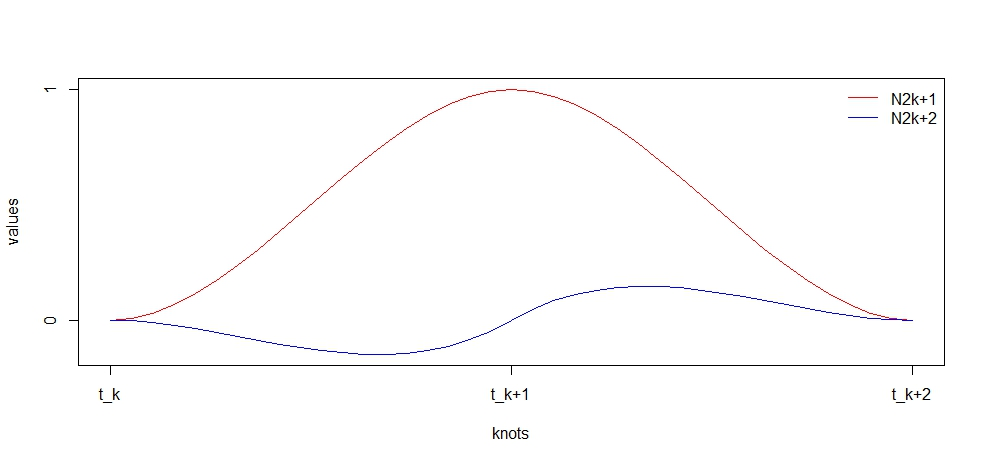
\includegraphics[width=\textwidth, height=9cm]{n2i}
\small \caption{The two basis functions $N_{2k+1}$ and $N_{2k+2}$ on interval $[t_k, t_{k+2}]$. It is apparently that these basis functions are continuous on this interval and have continuous first and second derivatives.}
\end{figure}

As independent basis functions, $N_1(t), \cdots, N_{2n}(t)$ span a $2n$ dimensional space $\mathbb{H}$. For any $f \in \mathbb{H}$, it is represented in the form of
\begin{equation}
f=\sum_{i=1}^{2n} \theta_i N_i(t).
\end{equation}

Suppose that we have observations $y_1,\cdots,y_n$ and $v_1,\cdots,v_n$. $f(t)$ can be found by minimizing equation (\ref{mse2}), which reduces to
\begin{equation}\label{tractormse}
\text{MSE}(\theta, \lambda,\gamma) = (\mathbf{y}-\mathbf{B}\theta)^\top (\mathbf{y}-\mathbf{B}\theta) +\gamma (\mathbf{v}-\mathbf{C}\theta)^\top (\mathbf{v}-\mathbf{C}\theta)+n\lambda \theta^\top\Omega\theta
\end{equation}
where $\{\mathbf{B}\}_{ij} = N_j(t_i)$ , $\{\mathbf{C}\}_{ij} = N'_j(t_i)$ and $\{\Omega_{2n} \}_{jk}=\int N''_j(t)N''_k(t)dt$. After substituting the series observation $t_1, \cdots, t_n$ into basis functions, we get $N_1(t_1)=1, N_1(t_2)=0, \cdots, N_{2k-1}(t_{k})=1, N_{2k}(t_{k})=0, \cdots, N_{2n-1}(t_n)=1, N_{2n}(t_n)=0$; and into first derivative of basis functions, we get $N'_1(t_1)=0, N_1'(t_2)=1, \cdots, N_{2k-1}'(t_{k})=0, N_{2k}'(t_{k})=1, \cdots, N_{2n-1}'(t_n)=0, N_{2n}'(t_n)=1$. That means the matrices $\mathbf{B}$ and $\mathbf{C}$ in MSE equation (\ref{tractormse}) are $n \times 2n$ dimensional and the elements are
\begin{align}
\mathbf{B}&=\{B\}_{ij}=\begin{cases}
1, & j=2i-1\\
0, & otherwise
\end{cases}\\
\mathbf{C}&=\{C\}_{ij}=\begin{cases}
1, & j=2i\\
0, & otherwise
\end{cases}
\end{align}
where $i=1, \cdots, n$.  Elements of penalty matrix $\{\Omega_{2n} \}_{jk}$ is given in appendices. 

The solution to (\ref{tractormse}) is easily seen to be
\begin{equation}\label{thetahat}
\hat{\theta}=(\mathbf{B}^\top\mathbf{B}+\gamma\mathbf{C}^\top\mathbf{C}+n\lambda\Omega)^{-1}(\mathbf{B}^\top\mathbf{y}+\gamma\mathbf{C}^\top\mathbf{v})
\end{equation}
a generalized ridge regression. Then the fitted smoothing spline is given by
\begin{equation}
\hat{f}(t)=\sum_{i=1}^{2n}N_i(t)\hat{\theta}_i
\end{equation}

A smoothing spline with parameters $\lambda$ and $\gamma$ is an example of a linear smoother \cite{esl2009}. This is because the estimated parameters in (\ref{thetahat}) are a linear combination of $y_i$ and $v_i$. Denote by $\hat{\mathbf{f}}$ the $2n$ vector of fitted values $\hat{f}(t_i)$ and $\hat{\mathbf{f}'}$ the $2n$ vector of fitted values $\hat{f'}(t_i)$ at the training points $t_i$. Then
\begin{equation}
\begin{split}
\hat{\mathbf{f}} =\mathbf{B}(\mathbf{B}^\top\mathbf{B}+\gamma\mathbf{C}^\top\mathbf{C}+n\lambda\Omega)^{-1}(\mathbf{B}^\top\mathbf{y}+\gamma\mathbf{C}^\top\mathbf{v})\\
\triangleq \mathbf{S}_{\lambda,\gamma}\mathbf{y}+\gamma\mathbf{T}_{\lambda,\gamma}\mathbf{v} 
\end{split}
\end{equation}
\begin{equation}
\begin{split}
\hat{\mathbf{f}'}
=\mathbf{C}(\mathbf{B}^\top\mathbf{B}+\gamma\mathbf{C}^\top\mathbf{C}+n\lambda\Omega)^{-1}(\mathbf{B}^\top\mathbf{y}+\gamma\mathbf{C}^\top\mathbf{v})\\
\triangleq\mathbf{U}_{\lambda,\gamma}\mathbf{y}+\gamma\mathbf{V}_{\lambda,\gamma}\mathbf{v}
\end{split}
\end{equation}
The fitted $\hat{\mathbf{f}}$ and $\hat{\mathbf{f}'}$ are linear in $\mathbf{y}$ and $\mathbf{v}$, and the finite linear operators $\mathbf{S}_{\lambda,\gamma}, \mathbf{T}_{\lambda,\gamma}, \mathbf{U}_{\lambda,\gamma}$ and $\mathbf{V}_{\lambda,\gamma}$ are known as the smoother matrices. One consequence of this linearity is that the recipe for producing $\hat{\mathbf{f}}$ and $\hat{\mathbf{f}'}$ from $\mathbf{y}$ and $\mathbf{v}$, do not depend on $\mathbf{y}$ and $\mathbf{v}$ themselves; $\mathbf{S}_{\lambda,\gamma}, \mathbf{T}_{\lambda,\gamma}, \mathbf{U}_{\lambda,\gamma}$ and $\mathbf{V}_{\lambda,\gamma}$ depend only on the $t_i,\lambda$ and $\gamma$.

Suppose in a traditional least squares fitting, $\mathbf{B}_\xi$ is $N \times M$ matrix of $M$ cubic-spline basis functions evaluated at the $N$ training points $x_i$, with knot sequence $\xi$ and $M \ll N$. Then the vector of fitted spline values is given by
\begin{align}\label{fhy}
\hat{\mathbf{f}}=\mathbf{B}_\xi(\mathbf{B}^\top_\xi\mathbf{B}_\xi)^{-1}\mathbf{B}_\xi\mathbf{y}=\mathbf{H}_\xi\mathbf{y}
\end{align}
Here the linear operator $\mathbf{H}_\xi$ is a symmetric, positive semidefinite matrices, and $\mathbf{H}_\xi\mathbf{H}_\xi=\mathbf{H}_\xi$ (idempotent). In our case, it is easily seen that $\mathbf{S}_{\lambda,\gamma}, \mathbf{T}_{\lambda,\gamma}, \mathbf{U}_{\lambda,\gamma}$ and $\mathbf{V}_{\lambda,\gamma}$ are symmetric, positive semidefinite matrices as well. However, only when $\lambda=\gamma=0$, the matrix $\mathbf{S}_{\lambda=0,\gamma=0}$ is idempotent.

\subsection{Tractor Spline Estimated by GP}

A tractor spline on interval $[t_1,t_n]$ has $2n$ basis functions $N_1(t), \cdots, N_{2n}(t)$, which are linear independent. So the space $\mathbb{H}$, spanned by these basis functions, is a $2n$ dimensional space. Following the  definition in section \ref{sectionRK}, it can be proved that the space $\mathbb{H}$ is a Reproducing Kernel Hilbert Space with inner product given in (\ref{innerproduct}), and kernel function $R(s,t)$ defined in (\ref{kernelfunction}).

Noticing the definition of Hermite Spline from equation (\ref{hermitebasis1}) to (\ref{hermitebasis4}), prior status of $y_i$ and $v_i$ will only affect the status $y_{i+1}$ and $v_{i+1}$ in the following time period $t_i$. Define a covariance matrix $\Lambda_i$ as 
\begin{align}
\Lambda_i = \text{cov}(\left[  \begin{matrix}y_i\\v_i\end{matrix}\right],\left[ \begin{matrix}y_{i+1}\\v_{i+1} \end{matrix}\right])
\end{align}
Then $f$ and $f'$ in $\mathbb{H}$ with zero mean Gaussian priors , have covariance functions
\begin{equation}
\begin{split}
\text{cov}(f(s),f(t))&=\tau^2 R(s,t)+\sigma_n^2\Lambda\\
\text{cov}(f(s),f'(t))&=\tau^2 R'(s,t)+\frac{\sigma_n^2}{\sqrt{\gamma}}\Lambda\\
\text{cov}(f'(s),f(t))&=\tau^2 \dot{R}(s,t)+\frac{\sigma_n^2}{\sqrt{\gamma}}\Lambda\\
\text{cov}(f'(s),f'(t))&=\tau^2 \dot{R}'(s,t)+\frac{\sigma_n^2}{\gamma}\Lambda
\end{split}
\end{equation}
Observing $y_i \sim N(f(t_i),\sigma_n^2)$ and $v_i \sim N(f'(t_i),\frac{\sigma_n^2}{\gamma})$, the joint distribution of $\mathbf{y}, \mathbf{v}, f(t)$ and $f'(t)$ is normal with zero mean and covariance matrix
\begin{equation}
\begin{split}
\text{cov}(\mathbf{y},\mathbf{v},f,f') =
\left[ \begin{matrix}
\tau^2Q+\sigma_n^2\Lambda & \tau^2 O+\frac{\sigma_n^2}{\sqrt{\gamma}}\Lambda & \tau^2\xi & \tau^2\xi' \\
\tau^2 O+\frac{\sigma_n^2}{\sqrt{\gamma}}\Lambda & \tau^2 P+\frac{\sigma_n^2}{\gamma}\Lambda & \tau^2 \dot{\xi}& \tau^2\dot{\xi}' \\
\tau^2\xi^\top & \tau^2\dot{\xi}^\top & \tau^2R(t,t)& \tau^2R'(t,t) \\
 \tau^2\xi'^\top& \tau^2\dot{\xi}'^\top& \tau^2\dot{R}(t,t)& \tau^2\dot{R}'(t,t)  \\
\end{matrix} \right]
\end{split}
\end{equation}
where $\{Q\}_{ij}$, $\{O\}_{ij}$, $\{P\}_{ij}$, $\xi$ and $\dot{\xi}$ are the same as that in (\ref{covyvff}). Then
\begin{equation}
\begin{split}
E\left[ \begin{matrix}
f \\
f'
\end{matrix} | \begin{matrix}
\mathbf{y} \\
\mathbf{v}
\end{matrix}\right] &= 
\left[ \begin{matrix}
\xi^\top& \dot{\xi}^\top \\
\xi'^\top & \dot{\xi}'^\top 
\end{matrix} \right] 
\left[ \begin{matrix}
Q+n\lambda \Lambda & O+\frac{n\lambda}{\sqrt{\gamma}} \Lambda\\
 O+\frac{n\lambda}{\sqrt{\gamma}} \Lambda &  P+\frac{n\lambda}{\gamma} \Lambda
\end{matrix} \right]^{-1}
\left[ 
\begin{matrix}
\mathbf{y} \\
\gamma \mathbf{v}
\end{matrix} \right] \\
&\triangleq
\left[ \begin{matrix}
\xi^\top& \dot{\xi}^\top \\
\xi'^\top & \dot{\xi}'^\top 
\end{matrix} \right] 
\left[ \begin{matrix}
A & B\\
C & D
\end{matrix} \right]
\left[ 
\begin{matrix}
\mathbf{y} \\
\gamma \mathbf{v}
\end{matrix} \right] \\
&=
\left[ \begin{matrix}
\xi^\top(A\mathbf{y}+B\gamma \mathbf{v})+ \dot{\xi}^\top(C\mathbf{y}+D\gamma \mathbf{v}) \\
\xi'^\top(A\mathbf{y}+B\gamma \mathbf{v})+ \dot{\xi}'^\top(C\mathbf{y}+D\gamma \mathbf{v}) 
\end{matrix} \right] 
\end{split}
\end{equation}
where $n\lambda = \sigma_n^2 / \tau^2$. The posterior mean is of the form $\xi^\top \mathbf{c}+\dot{\xi}^\top\mathbf{d}$, and $E(f' | \mathbf{y},\mathbf{v})$ is of the form $\xi'^\top \mathbf{c}+\dot{\xi}'^\top\mathbf{d}$, with the same coefficients given by
\begin{align}
\mathbf{c}&=A\mathbf{y}+B\gamma \mathbf{v}\\
\mathbf{d}&=C\mathbf{y}+D\gamma \mathbf{v} 
\end{align}


Following the procedure in section \ref{sectionRK} and \ref{secmatrixandmean}, we use observations $t_i, i=1, \cdots, n$ to construct a subspace $\mathbb{A}\subset\mathbb{H}$, which is a linear combination of kernel functions $R(s,t)$, as
\begin{equation}
\mathbb{A}=\{f: f=\sum_{i=1}^{n}\alpha_iR(t_i,\cdot)\}.
\end{equation}

The covariance matrix and posterior mean all given above, and the solution can be computed via finding $\mathbf{c}$ and $\mathbf{d}$.

In fact, for a tractor spline, the space $\mathbb{A}$ only contains terms of odd basis functions $N_{2k-1}$, which can be seen from matrix $\mathbf{B}$ in (\ref{tractormse}). So we construct another subspace
\begin{equation}
\mathbb{B}=\{f: f=\sum_{i=1}^{n}\beta_i \dot{R}(t_i,\cdot)=\sum_{i=1}^{n}\alpha_i \sum_{j=1}^{2n}N'_j(t_i)N_j(\cdot)\} 
\end{equation}
where $\dot{R}$ is defined in equation (\ref{dotr}). This subspace contains even terms basis functions $N_{2k}$. So $\mathbb{A} \cap \mathbb{B} = \emptyset$. 

Thus $f \in \mathbb{H}$ can be written as
\begin{equation}\label{etaeq3}
f(t)=\sum_{i=1}^{n}c_iR(t_i,t)+\sum_{i=1}^{n}d_i \dot{R}(t_i,t)+\rho(t)
\end{equation}
where $c_i, d_i$ are coefficients, $\rho(t) \in \mathbb{H} \ominus (\mathbb{A} \oplus \mathbb{B})$, and 
\begin{equation}\label{etaeq4}
f'(t)=\sum_{i=1}^{n}c_iR'(t_i,t)+\sum_{i=1}^{n}d_i \dot{R}'(t_i,t)+\rho'(t).
\end{equation}

The equation (\ref{mse2}) can be written as
\begin{equation}
\begin{split}
&\frac{1}{n}\sum_{i=1}^n (y_i -\sum_{j=1}^{n}c_jR(t_j,t_i)- \sum_{j=1}^{n}d_j\dot{R}(t_j,t_i) -\rho(t_i))^2\\
+&\frac{\gamma}{n}\sum_{i=1}^n (v_i -\sum_{j=1}^{n}c_jR'(t_j,t_i)- \sum_{j=1}^{n}d_j\dot{R}'(t_j,t_i) -\rho'(t_i))^2\\
+&\lambda \int_{t_1}^{t_n} (\sum_{j=1}^{n}c_jR''(t_j,t)+ \sum_{j=1}^{n}d_j\dot{R}''(t_j,t) +\rho''(t))^2dt
\end{split}
\end{equation}
By orthogonality, $\rho(t_i) = \langle R(t_i,\cdot),\rho\rangle=0$, %$\rho(t_i) =\langle\rho,R'(\cdot,t_i)\rangle=\langle\dot{R}(t_i,\cdot),\rho\rangle=0$, 
and $\rho'(t_i) = \langle\dot{R}(t_i,\cdot),\rho\rangle=0$, where $i=1,\cdots,n$. 

Denoting by $Q$ the $n \times n$ matrix with the $(i,j)$th entry $R(t_i,t_j)$, by $P$ the $n \times n$ matrix with the $(i,j)$th entry $\dot{R}(t_i,t_j)$ the equation (\ref{tractormse}) can be written as
\begin{equation}\label{matrixeq}
(\mathbf{y}-Q\mathbf{c}-P\mathbf{d})^\top(\mathbf{y}-Q\mathbf{c}-P\mathbf{d})+\gamma (\mathbf{v}-\frac{\partial Q}{\partial t}\mathbf{c}-\frac{\partial P}{\partial t}\mathbf{d})^\top(\mathbf{v}-\frac{\partial Q}{\partial t}\mathbf{c}-\frac{\partial P}{\partial t}\mathbf{d})+n\lambda \Omega+\lambda(\rho,\rho).
\end{equation}
The elements of penalty matrix $\Omega$ is in appendices. Note that $\rho$ only appears in the third term in $(\ref{matrixeq})$, which is minimized at $\rho=0$. Hence, a polynomial smoothing spline resides in the space $\mathbb{A} \oplus \mathbb{B}$ of finite dimension. Then the solution could be computed via minimization of term in $(\ref{matrixeq})$ with respect to $\mathbf{c}$ and $\mathbf{d}$.

\section{Cross Validation}

The coefficients can be calculated by minimizing MSE function. While another problem is how to choose smoothing parameter. There are two different philosophical approaches to the question of choosing the smoothing parameter. The first approach is to regard the free choice of smoothing parameter as an advantageous feature of the procedure. The other is a need for an automatic method whereby the smoothing parameter values is chose by the data, \cite{green1993nonparametric}. 

Assuming that the random error has zero mean, the true regression curve $f$ has the property that, if an observation $y$ is taken at a point $t$, the value $f(t)$ is the best predictor of $y$ in terms of returning a small value of $(y-f(t))^2$. 

Now we focus on an observation $y_i$ at point $t_i$ as being a new observation by omitting it from the set of data, which are used to estimate $\hat{f}$. Denote by $\hat{f}^{(-i)}(t,\lambda)$ the estimated function from the remaining data, where $\lambda$ is the smoothing parameter. Then $\hat{f}^{(-i)}(t,\lambda)$ minimizes 
\begin{align}
\frac{1}{n}\sum_{j \neq i}(y_j-f(t_j))^2+\lambda \int f''^2dt
\end{align}
 and $\lambda$ can be quantified by cross-validation score function
\begin{align}
CV(\lambda)=\frac{1}{n}\sum_{i=1}^{n}\{y_i-\hat{f}^{(-i)}(t_i,\lambda)\}^2.
\end{align}
The basis idea of cross-validation is to choose the value of $\lambda$ that minimizes $CV(\lambda)$. 

An efficient way to calculate cross validation score is given by \cite{green1993nonparametric}. Through the equation (\ref{fhy}), we know that the value of the smoothing spline $\hat{f}$ depend linearly on the data $y_i$. Define the matrix $A(\lambda)$, which is a map vector of observed values $y_i$ to predicted values $\hat{f}(t_i)$. Then we have
\begin{equation}
\mathbf{f}=A(\lambda)\mathbf{y}
\end{equation}
and the following lemma.
\begin{lemma}
The cross validation score satisfies
\begin{equation}
CV(\lambda)=\frac{1}{n} \sum_{i=1}^n(\frac{y_i-\hat{f}(t_i)}{1-A_{ii}(\lambda)})^2
\end{equation}
where $\hat{f}$ is the spline smoother calculated from the full data set $\{(t_i,y_i)\}$ with smoothing paramter $\lambda$.
\end{lemma}

For a tractor spline and its MSE function, there are two parameters need to be estimated $\lambda$ and $\gamma$. Thus the objective function becomes
\begin{align}
\frac{1}{n}\sum_{j \neq i}(y_j-f(t_j))^2+\frac{\gamma}{n}\sum_{j \neq i}(v_j-f'(t_j))^2+\lambda \int f''^2dt,
\end{align}
and the cross-validation score function is
\begin{align}
CV(\lambda,\gamma)=\frac{1}{n}\sum_{i=1}^{n}\{y_i-\hat{f}^{(-i)}(t_i,\lambda,\gamma)\}^2.
\end{align}

For a tractor spline, the parameter $\hat{\theta}=(B^\top B+\gamma C^\top C+n\Omega_\lambda)^{-1}(B^\top\mathbf{y}+\gamma C^\top\mathbf{v})$, then
\begin{equation}
\begin{split}
 \hat{f}&=B\hat{\theta}=B(B^\top B+\gamma C^\top C+n\Omega_\lambda)^{-1}B^\top\mathbf{y}+B(B^\top B+\gamma C^\top C+n\Omega_\lambda)^{-1}C^\top\mathbf{v}\\&=S\mathbf{y}+\gamma T\mathbf{v},
 \end{split}
 \end{equation}
 \begin{equation}
 \begin{split}
\hat{f}'&=C\hat{\theta}=C(B^\top B+\gamma C^\top C+n\Omega_\lambda)^{-1}B^\top\mathbf{y}+C(B^\top B+\gamma C^\top C+n\Omega_\lambda)^{-1}C^\top\mathbf{v}\\&=U\mathbf{y}+\gamma V\mathbf{v}.
 \end{split}
\end{equation}
Then 
\begin{theorem}\label{cvscore}
The cross validation score of a tractor spline satisfies
\begin{equation}
CV(\lambda,\gamma)=\frac{1}{n}\sum_{i=1}^{n}\frac{\hat{f}(t_i)-y_i+\gamma \frac{T_{ii}}{1-\gamma V_{ii}}(\hat{f}'(t_i)-v_i)}{1-S_{ii}-\gamma\frac{T_{ii}}{1-\gamma V_{ii}}U_{ii}}
\end{equation}
where $\hat{f}$ is the tractor spline smoother calculated from the full data set $\{(t_i,y_i,v_i)\}$ with smoothing paramter $\lambda$ and $\gamma$.
\end{theorem}

The proof of Theorem \ref{cvscore} follows immediately from a lemma, and gives an expression for the deleted residuals $y_i-\hat{f}^{(-i)}(t_i)$ and $v_i-\hat{f}'^{(-i)}(t_i)$ in terms of $y_i-\hat{f}(t_i)$ and $v_i-\hat{f}'(t_i)$ respectively. 

\begin{lemma} \label{cvlemma}
For fixed $\lambda,\gamma$ and $i$, denote $\mathbf{f}^{(-i)}$ by the vector with components $f_j^{(-i)}=\hat{f}^{(-i)}(t_j,\lambda,\gamma)$,  $\mathbf{f}'^{(-i)}$ by the vector with components $f_j'^{(-i)}=\hat{f}'^{(-i)}(t_j,\lambda,\gamma)$, and define vectors $\mathbf{y}^*$ and $\mathbf{v}^*$ by 
\begin{align}
\begin{cases}
y_j^*=y_j &j \neq i\\
y_i^*=\hat{f}^{(-i)}(t_i) &otherwise
\end{cases},\\
\begin{cases}
v_j^*=v_j &j \neq i\\
v_i^*=\hat{f}'^{(-i)}(t_i) &otherwise
\end{cases}.
\end{align}
Then
\begin{align}
\mathbf{\hat{f}}^{(-i)}&=S\mathbf{y}^*+\gamma T\mathbf{v}^*\\
\mathbf{\hat{f}}'^{(-i)}&=U\mathbf{y}^*+\gamma V\mathbf{v}^*
\end{align}
\end{lemma}

\subsection{K-Fold Cross Validation}

Based on the procedure given by \cite{wahba1975completely}, we  follow the improved steps to calculate a K-fold cross validation. 

Step 1. Remove the first data $t_1$ and last date $t_n$ from the dataset.

Step 2. Divide dataset into k groups:
\begin{align*}
& \mbox{Group 1}: t_2, t_{2+k}, \cdots \\
& \mbox{Group 2}: t_3, t_{3+k}, \cdots \\
& \vdots \\
& \mbox{Group k}: t_{k+1}, t_{2k+1}, \cdots
\end{align*}


Step 3. Guess values of $\lambda_{down}, \lambda_{up}$ and $\gamma$.

Step 4. Delete the first group of data. Fit a smoothing spline to the first data, the rest groups of dataset and the last data, with  $\lambda_{down}, \lambda_{up}$ and $\gamma$ in step 3. Compute the sum of squared deviations of this smoothing spline from the deleted data points.

Step 5. Delete instead the second group of data. Fit a smoothing spline to the remaining data with  $\lambda_{down}, \lambda_{up}$ and $\gamma$. Compute the sum of squared deviations of the spline from deleted data points.

Step 6. Repeat Step 5 for the 3rd, 4th, $\cdots$, $k$th group of data.

Step 7. Add the sums of squared deviations from steps 4 to 6 and divide by $k$. This is the cross validation score of three parameters  $\lambda_{down}, \lambda_{up}$ and $\gamma$.

Step 8. Vary  $\lambda_{down}, \lambda_{up}$ and $\gamma$ systematically and repeat steps 4-7 until CV shows a minimum.
